\input{../preamble.tex}

\lecturenumber{8}
\title{Advanced Scheduling}
\version{2.0.0}

\begin{document}
  \begin{frame}[plain, noframenumbering]
    \titlepage
  \end{frame}

\begin{slide}

	\slidetitle{How to schedule without perfect knowledge?}
	
	How can we design a scheduler system that both
	\begin{itemize}
		\item minimizes response time for interactive jobs
		\item minimizes turnaround time without a priori knowledge of job length
	\end{itemize}
	\bigskip
	
	We may favor some processes over others.
	
\end{slide}

\begin{slide}

	\slidetitle{Multi-level Feedback Queue (MLFQ)} 
	
	There are multiple queues with different priority levels.
	\begin{itemize}
		\item If Priority(A) > Priority(B), A runs (B doesn't).
		\item If Priority(A) = Priority(B), A and B run in RR.
	\end{itemize}
	\bigskip
	
\end{slide}

\begin{slide}

	\slidetitle{A Snapshop of MLFQ}
	
	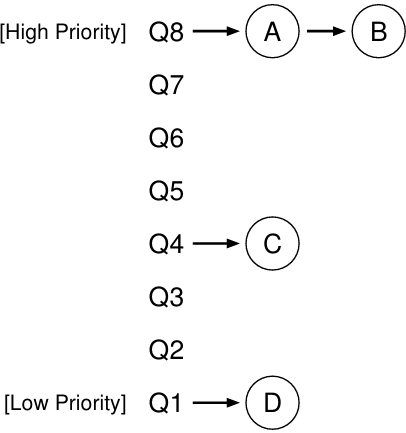
\includegraphics[width=50mm]{snapshot-mlfq.png}
	
\end{slide}

\begin{slide}

	\slidetitle{Dynamic Priority}
	
	We may lead processes to \textit{starvation} if there's a lot of higher
    priority processes
    \bigskip
	
	One solution is to have the OS dynamically change the priority
	
\end{slide}

\begin{slide}

	\slidetitle{Dynamic Priority Attempt 1}
	
	New jobs are placed at the top queue with highest priority.
	\bigskip
	
	Allotment: Each job is allocated a time slice before the scheduler reduces its priority.
	\bigskip
	
	If a job uses up its allotment while running, its priority is reduced.
	\bigskip
	
	A job's usage resets if it gives up the CPU before its allotted time is used up.

\end{slide}

\begin{slide}

	\slidetitle{Dynamic Priority Attempt 1}
	
	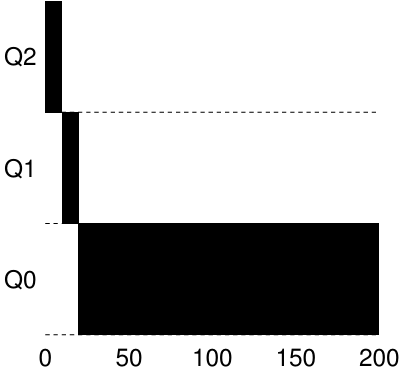
\includegraphics[width=60mm]{MLFQ-1-EX-1.png}

\end{slide}

\begin{slide}

	\slidetitle{Dynamic Priority Attempt 1}
	
	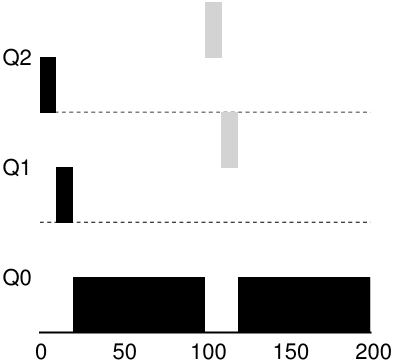
\includegraphics[width=60mm]{MLFQ-1-EX-2.png}

\end{slide}

\begin{slide}

	\slidetitle{Dynamic Priority Attempt 1}
	
	Prioritizes I/O-intensive interactive jobs (good response time).
	\bigskip
	
	Can cause starvation.
	\bigskip
	
	Users can try to cheat the system.
	\bigskip
	
	What if a long-running program becomes interactive later?

\end{slide}

\begin{slide}

	\slidetitle{Dynamic Priority Attempt 2}
	
	After some time period \texttt{S}, move all the jobs in the system to the topmost queue.
	\bigskip
	
	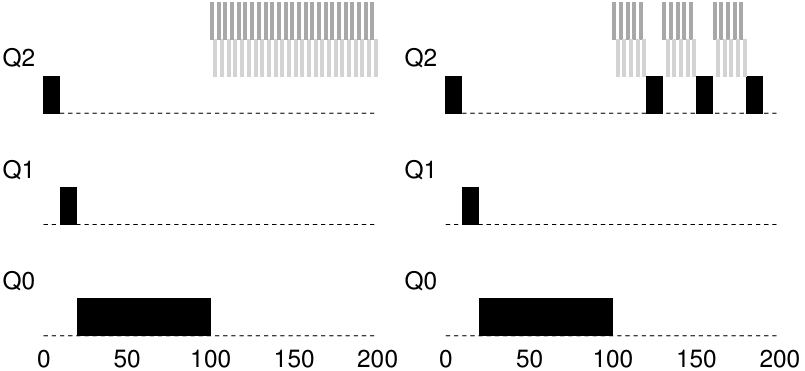
\includegraphics[width=100mm]{MLFQ-2-EX-1.PNG}
	
\end{slide}

\begin{slide}

	\slidetitle{Dynamic Priority Attempt 3}
	
	A job's usage \textbf{does not reset} if it gives up the CPU before its allotted time is used up.
	\bigskip
	
	How many queues?
	\bigskip
	
	How long is an allotment?
	\bigskip
	
	How long is the time period \texttt{S}?
	
\end{slide}

  \begin{slide}

    \slidetitle{Scheduling Can Get Complicated}

    There's no ``right answer'', only trade-offs
    \medskip

    We haven't talked about multiprocessor scheduling yet
    \medskip

    We'll assume symmetric multiprocessing (SMP)

    \leftspace{}All CPUs are connected to the same physical memory

    \leftspace{}The CPUs have their own private cache (at least the lowest levels)

  \end{slide}

  \begin{slide}

    \slidetitle{One Approach is to Use the Same Scheduling for All CPUs}

    There's still only one scheduler

    \leftspace{}It just keeps adding processes while there's available CPUs
    \medskip

    Advantages

    \leftspace{}Good CPU utilization

    \leftspace{}Fair to all processes
    \medskip

    Disadvantages

    \leftspace{}Not scalable (everything blocks on global scheduler)

    \leftspace{}Poor cache locality
    \medskip

    This was the approach in Linux 2.4

  \end{slide}

  \begin{slide}

    \slidetitle{We Can Create Per-CPU Schedulers}

    When there's a new process, assign it to a CPU

    \leftspace{}One strategy is to assign it to the CPU with the lowest number of processes
    \medskip

    Advantages

    \leftspace{}Easy to implement

    \leftspace{}Scalable (there's no blocking on a resource)

    \leftspace{}Good cache locality
    \medskip

    Disadvantages

    \leftspace{}Load imbalance

    \leftspace{}\leftspace{}Some CPUs may have less processes, or less intensive ones

  \end{slide}

  \begin{slide}

    \slidetitle{We Can Compromise between Global and Per-CPU}

    Keep a global scheduler that can rebalance per-CPU queues

    \leftspace{}If a CPU is idle, take a process from another CPU (work stealing)
    \medskip

    You may want more control over which processes can switch

    \leftspace{}Some may be more sensitive to caches
    \medskip

    Use \textit{processor affinity}

    \leftspace{}The preference of a process to be scheduled on the same core
    \medskip

    This is a simplified version of the O(1) scheduler in Linux 2.6

  \end{slide}


  \begin{slide}

    \slidetitle{Real-Time Scheduling is Yet Another Problem}

    Real-time means there are time constraints, either for a deadline or rate

    \leftspace{}e.g. audio, autopilot
    \medskip

    A hard real-time system

    \leftspace{}Required to guarantee a task completes within a certain amount
    of time
    \medskip

    A soft real-time system

    \leftspace{}Critical processes have a higher priority and the deadline is
    met in practice
    \medskip

    Linux is an example of soft real-time

  \end{slide}

  \begin{slide}

    \slidetitle{Linux Also Implements FCFS and RR Scheduling}

    You can search the source tree: FCFS (\texttt{SCHED\_FIFO}) and RR (\texttt{SCHED\_RR})
    \medskip

    Use a multilevel queue scheduler for processes with the same priority

    \leftspace{}Also let the OS dynamically adjust the priority
    \medskip

    Soft real-time processes:

    \leftspace{}Always schedule the highest priority processes first
    \medskip

    Normal processes:

    \leftspace{}Adjust the priority based on aging

  \end{slide}

  \begin{slide}

    \slidetitle{Real-Time Processes Are Always Prioritized}

    The soft real-time scheduling policy will either be \texttt{SCHED\_FIFO}
    or \texttt{SCHED\_RR}

    \leftspace{}There are 100 static priority levels (0---99)
    \medskip

    Normal scheduling policies apply to the other processes
    (\texttt{SCHED\_NORMAL})

    \leftspace{}By default the priority is 0

    \leftspace{}Priority ranges from $\mathsf{[-20, 19]}$
    \medskip

    Processes can change their own priorities with system calls:

    \leftspace{}\texttt{nice}, \texttt{sched\_setscheduler}

  \end{slide}

  \begin{slide}
    
    \slidetitle{Linux Priority Unifies Soft Real-time and Normal Processes}

    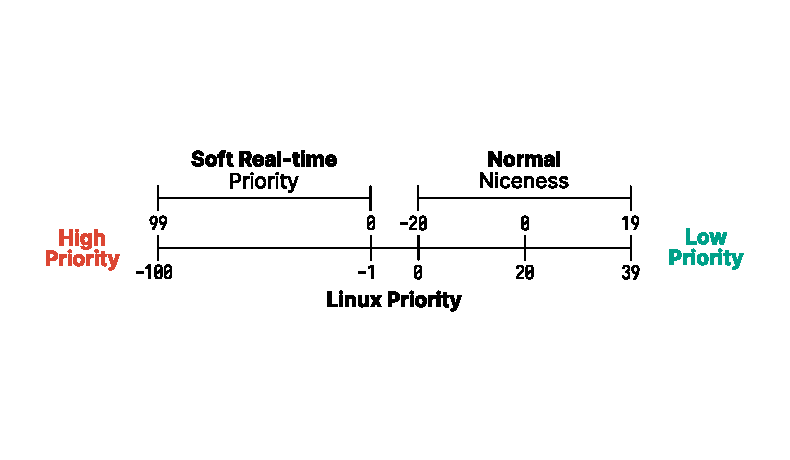
\includegraphics{linux-priority.eps}

  \end{slide}

  \begin{slide}

    \slidetitle{Linux Scheduler Evolution}

    2.4---2.6, a $\mathsf{O(N)}$ global queue

    \leftspace{}Simple, but poor performance with multiprocessors and many processes
    \medskip

    2.6---2.6.22, a per-CPU run queue, $\mathsf{O(1)}$ scheduler

    \leftspace{}Complex to get right, interactivity had issues

    \leftspace{}No guarantee of fairness
    \medskip

    2.6.23---Present, the completely fair scheduler (CFS)

    \leftspace{}Fair, and allows for good interactivity

  \end{slide}

  \begin{slide}

    \slidetitle{The $\mathsf{O(1)}$ Scheduler Has Issues with Modern Processes}

    Foreground and background processes are a good division

    \leftspace{}Easier with a terminal, less so with GUI processes
    \medskip

    Now the kernel has to detect interactive processes with heuristics

    \leftspace{}Processes that sleep a lot may be more interactive

    \leftspace{}\leftspace{}This is ad hoc, and could be unfair
    \medskip

    How would we introduce fairness for different priority processes?

    \leftspace{}Use different size time slices

    \leftspace{}The higher the priority, the larger the time slice

    \leftspace{}\leftspace{}There are also situations where this ad hoc solution
    could be unfair

  \end{slide}

  \begin{slide}

    \slidetitle{Ideal Fair Scheduling}

    Assume you have an infinitely small time slice

    \leftspace{}If you have $\mathsf{n}$ processes, each runs at $\mathsf{\frac{1}{n}}$ rate
    \medskip

    \begin{tikzpicture}
      \draw (0, 6em) rectangle (30em, 7.5em);

      \node [anchor=east] at (0, 6.75em) {1 Process};

      \draw (0, 3.5em) rectangle (10em, 5em);
      \draw (0, 1.75em) rectangle (10em, 3.25em);
      \draw (0, 0) rectangle (10em, 1.5em);

      \node [anchor=east] at (0, 2.5em) {3 Processes};
    \end{tikzpicture}
    \bigskip

    CPU usage is divided equally among every process

  \end{slide}

  \begin{slide}

    \slidetitle{Example IFS Scheduling}

    Consider the following processes:

    \begin{center}
      \footnotesize
      \begin{tabular}{lrr}
        Process & Arrival Time & Burst Time \\
        $\mathsf{P_1}$ & 0 & 8 \\
        $\mathsf{P_2}$ & 0 & 4 \\
        $\mathsf{P_3}$ & 0 & 16 \\
        $\mathsf{P_4}$ & 0 & 4 \\
      \end{tabular}
    \end{center}

    Assume that each vertical slice can execute 4 time units.

    \leftspace{}Each box represents the time units spend executing

    \begin{center}
      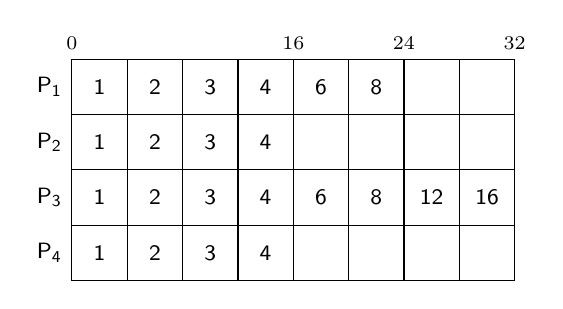
\begin{tikzpicture}

        %% \fill [black!80] (0,0) rectangle (14em, 2em);

        %% \fill [black!60] (14em,0) rectangle (22em, 2em);

        %% \fill [black!40] (22em,0) rectangle (24em, 2em);

        %% \fill [black!20] (24em,0) rectangle (32em, 2em);

        \draw (0,0) rectangle (16em,8em);

        \foreach \i in {1,...,7} {
          \draw [shorten >=0] (\i * 2em, 0) -- (\i * 2em, 8em);
        }

        \foreach \i in {1,...,3} {
          \draw [shorten >=0] (0, \i * 2em) -- (16em, \i * 2em);
        }

        \node [anchor=east] at (0, 7em) {\footnotesize $\mathsf{P_1}$};
        \node [anchor=east] at (0, 5em) {\footnotesize $\mathsf{P_2}$};
        \node [anchor=east] at (0, 3em) {\footnotesize $\mathsf{P_3}$};
        \node [anchor=east] at (0, 1em) {\footnotesize $\mathsf{P_4}$};

        \node at (1em, 7em) {\footnotesize $\mathsf{1}$};
        \node at (1em, 5em) {\footnotesize $\mathsf{1}$};
        \node at (1em, 3em) {\footnotesize $\mathsf{1}$};
        \node at (1em, 1em) {\footnotesize $\mathsf{1}$};

        \node at (3em, 7em) {\footnotesize $\mathsf{2}$};
        \node at (3em, 5em) {\footnotesize $\mathsf{2}$};
        \node at (3em, 3em) {\footnotesize $\mathsf{2}$};
        \node at (3em, 1em) {\footnotesize $\mathsf{2}$};

        \node at (5em, 7em) {\footnotesize $\mathsf{3}$};
        \node at (5em, 5em) {\footnotesize $\mathsf{3}$};
        \node at (5em, 3em) {\footnotesize $\mathsf{3}$};
        \node at (5em, 1em) {\footnotesize $\mathsf{3}$};

        \node at (7em, 7em) {\footnotesize $\mathsf{4}$};
        \node at (7em, 5em) {\footnotesize $\mathsf{4}$};
        \node at (7em, 3em) {\footnotesize $\mathsf{4}$};
        \node at (7em, 1em) {\footnotesize $\mathsf{4}$};

        \node at (9em, 7em) {\footnotesize $\mathsf{6}$};
        \node at (9em, 3em) {\footnotesize $\mathsf{6}$};

        \node at (11em, 7em) {\footnotesize $\mathsf{8}$};
        \node at (11em, 3em) {\footnotesize $\mathsf{8}$};

        \node at (13em, 3em) {\footnotesize $\mathsf{12}$};

        \node at (15em, 3em) {\footnotesize $\mathsf{16}$};

        \node [anchor=south] at (0em, 8em) {\scriptsize 0};
        \node [anchor=south] at (8em, 8em) {\scriptsize 16};
        \node [anchor=south] at (12em, 8em) {\scriptsize 24};
        \node [anchor=south] at (16em, 8em) {\scriptsize 32};
      \end{tikzpicture}
    \end{center}

  \end{slide}

  \begin{slide}

    \slidetitle{IFS is the Fairest but Impractical Policy}

    This policy is fair, every process gets an equal amount of CPU time

    \leftspace{}Boosts interactivity, has the ideal response time
    \medskip

    However, this would perform way too many context switches
    \medskip

    You have to constantly scan all processes, which is $\mathsf{O(N)}$

  \end{slide}

  \begin{slide}

    \slidetitle{Completely Fair Scheduler (CFS)}

    For each runnable process, assign it a ``virtual runtime''

    \leftspace{}At each scheduling point where the process runs for time \texttt{t}

    \leftspace{}\leftspace{}Increase the virtual runtime by \texttt{t}
    $\mathsf{\times}$ weight (based on priority)
    \medskip

    The virtual runtime monotonically increases

    \leftspace{}Scheduler selects the process based on the lowest virtual runtime

    \leftspace{}\leftspace{}Compute its dynamic time slice based on the IFS
    \medskip

    Allow the process to run, when the time slice ends repeat the process

  \end{slide}

  \begin{slide}

    \slidetitle{CFS is Implemented with Red-Black Trees}

    A red-black tree is a self-balancing binary search tree

    \leftspace{}Keyed by virtual runtime

    \leftspace{}\leftspace{}$\mathsf{O(lg N)}$ insert, delete, update, find
    minimum
    \medskip

    The implementation uses a red-black tree with nanosecond granularity

    \leftspace{}Doesn't need to guess the interactivity of a process
    \medskip

    CFS tends to favour I/O bound processes by default

    \leftspace{}Small CPU bursts translate to a low virtual runtime

    \leftspace{}\leftspace{}It will get a larger time slice, in order to catch
    up to the ideal

  \end{slide}

\end{document}
